%!TEX TS-program = xelatex
\documentclass[a4paper]{friggeri-cv}
\usepackage{afterpage}
\usepackage{hyperref}
\usepackage{color}
\usepackage{xcolor}
\usepackage{smartdiagram}
\usepackage{fontspec}


% if you want to add fontawesome package
% you need to compile the tex file with LuaLaTeX
% References:
%   http://texdoc.net/texmf-dist/doc/latex/fontawesome/fontawesome.pdf
%   https://www.ctan.org/tex-archive/fonts/fontawesome?lang=en
%\usepackage{fontawesome}
\usepackage{metalogo}
\usepackage{dtklogos}
\usepackage[utf8]{inputenc}
\usepackage{tikz}
\usetikzlibrary{mindmap,shadows}
\hypersetup{
    pdftitle={},
    pdfauthor={},
    pdfsubject={},
    pdfkeywords={},
    colorlinks=false,           % no lik border color
    allbordercolors=white       % white border color for all
}
\smartdiagramset{
    bubble center node font = \footnotesize,
    bubble node font = \footnotesize,
    % specifies the minimum size of the bubble center node
    bubble center node size = 0.5cm,
    %  specifies the minimum size of the bubbles
    bubble node size = 0.5cm,
    % specifies which is the distance among the bubble center node and the other bubbles
    distance center/other bubbles = 0.3cm,
    % sets the distance from the text to the border of the bubble center node
    distance text center bubble = 0.5cm,
    % set center bubble color
    bubble center node color = pblue,
    % define the list of colors usable in the diagram
    set color list = {lightgray, materialcyan, orange, green, materialorange, materialteal, materialamber, materialindigo, materialgreen, materiallime},
    % sets the opacity at which the bubbles are shown
    bubble fill opacity = 0.6,
    % sets the opacity at which the bubble text is shown
    bubble text opacity = 0.5,
}

\addbibresource{bibliography.bib}
\RequirePackage{xcolor}
\definecolor{pblue}{HTML}{0395DE}

\begin{document}
\header{Ali}{Heydari}
      {Computer Engineer}

% Fake text to add separator
\fcolorbox{white}{gray}{\parbox{\dimexpr\textwidth-2\fboxsep-2\fboxrule}{%
.....
}}

% In the aside, each new line forces a line break
\begin{aside}
  \includegraphics[scale=0.025]{img/Ali_Heydari.jpg}
  \section{Address}
Iran- Tehran- Narmak -
Iran University of Science and Technology.
    ~
  \section{Tel \& Skype}
   \href{tel:+989368563509}{+98 936 856 3509}
    ~
  \section{Mail}
 \href{mailto:ali4heydari@gmail.com}{\textbf{ali4heydari@}\\gmail.com}
    ~
  \section{Web \& Git}
     \href{https://github.com/ali4heydari}{github.com/ali4heydari}
    \href{https://gitlab.com/u/ali4heydari}{gitlab.com/u/ali4heydari}
    ~
  % use  \hspace{} or \vspace{} to change bubble size, if needed
  \section{Programming}
   \smartdiagram[bubble diagram]{
        \textbf{C/C++},
        \textbf{Python},
        \textbf{Java},
       % \textbf{Lua/UCI},
        %\textbf{Other\vspace{3mm}},
        %\textbf{HTML/CSS}\\\textbf{JS/jQuery},
       % \textbf{PHP},
        %\textbf{Android},
        \textbf{C\#}
    }
    ~
  \section{Personal Skills}
    \smartdiagram[bubble diagram]{
        \textbf{Team}\\\textbf{Player},
        \textbf{Initiative},
        \textbf{Curiosity},
        \textbf{Problem}\\\textbf{Solving},
        \textbf{\vspace{2mm}Manage\vspace{2mm}},
        \textbf{Organize}
    }
    ~
\end{aside}
~
\section{Experience}
\begin{entrylist}
  \entry
    {01/18 - Now}
    {Security expert}
    {AmnGostar Co}
    {TEXT HERE\\}
  \entry
    {10/17 - 04/18}
    {Teacher \& Lesson Officer }
    {Kanoon Farhangi Amoozesh}
    {TEXT HERE\\}
  \entry
    {09/17 - 07/17}
    {TABESH Cultural Group}
    {Sharif University of Technology}
        {TEXT HERE\\}
    \entry
    {09/17 - 07/17}
    {Member of the Kimia Student Practical Group}
    {Sharif University of Technology}
    {TEXT HERE\\}
    \entry
    {02/11 - 02/11}
    {Participation in calligraphy exhibition NOGHTE}
    {Association of the Calligraphers of Delijan}
    {TEXT HERE}
    \entry
        {02/08 - 06/10}
    {Memmber of association of Calligraphers of Delijan}
    {Association of the Calligraphers of Delijan}
    {TEXT HERE}
\end{entrylist}
\\
\section{Education}
\begin{entrylist}
  \entry
    {2017 - Now}
    {B.Sc in Computer Engineering}
    {Iran University of Science and Technology}
    {Lorem ipsum dolor sit amet, consectetur adipiscing elit, sed do eiusmod tempor incididunt ut labore et dolore magna aliqua. Ut enim ad minim veniam, quis nostrud exercitation ullamco laboris nisi ut aliquip ex ea commodo consequat\\}
  \entry
    {2016 - 2017}
    {B.Sc in Chemical Engineering}
    {Shari University of Technology}
    {Lorem ipsum dolor sit amet, consectetur adipiscing elit, sed do eiusmod tempor incididunt ut labore et dolore magna aliqua. Ut enim ad minim veniam, quis nostrud exercitation ullamco laboris nisi ut aliquip ex ea commodo consequat\\}
  \entry
    {2011 - 2015}
    {Scientific Disploma}
    {Beheshti Highschool}
    {}
\end{entrylist}

\newpage

\begin{aside}
~
~
~
  \section{OS Preference}
    \textbf{GNU/Linux}
\includegraphics[scale=0.40]{img/5stars.png}
    \textbf{Unix}
\includegraphics[scale=0.40]{img/4stars.png}
    \textbf{MacOS}
\includegraphics[scale=0.40]{img/2stars.png}
    \textbf{Windows}
\includegraphics[scale=0.40]{img/1stars.png}
    ~
  \section{Places Lived}
    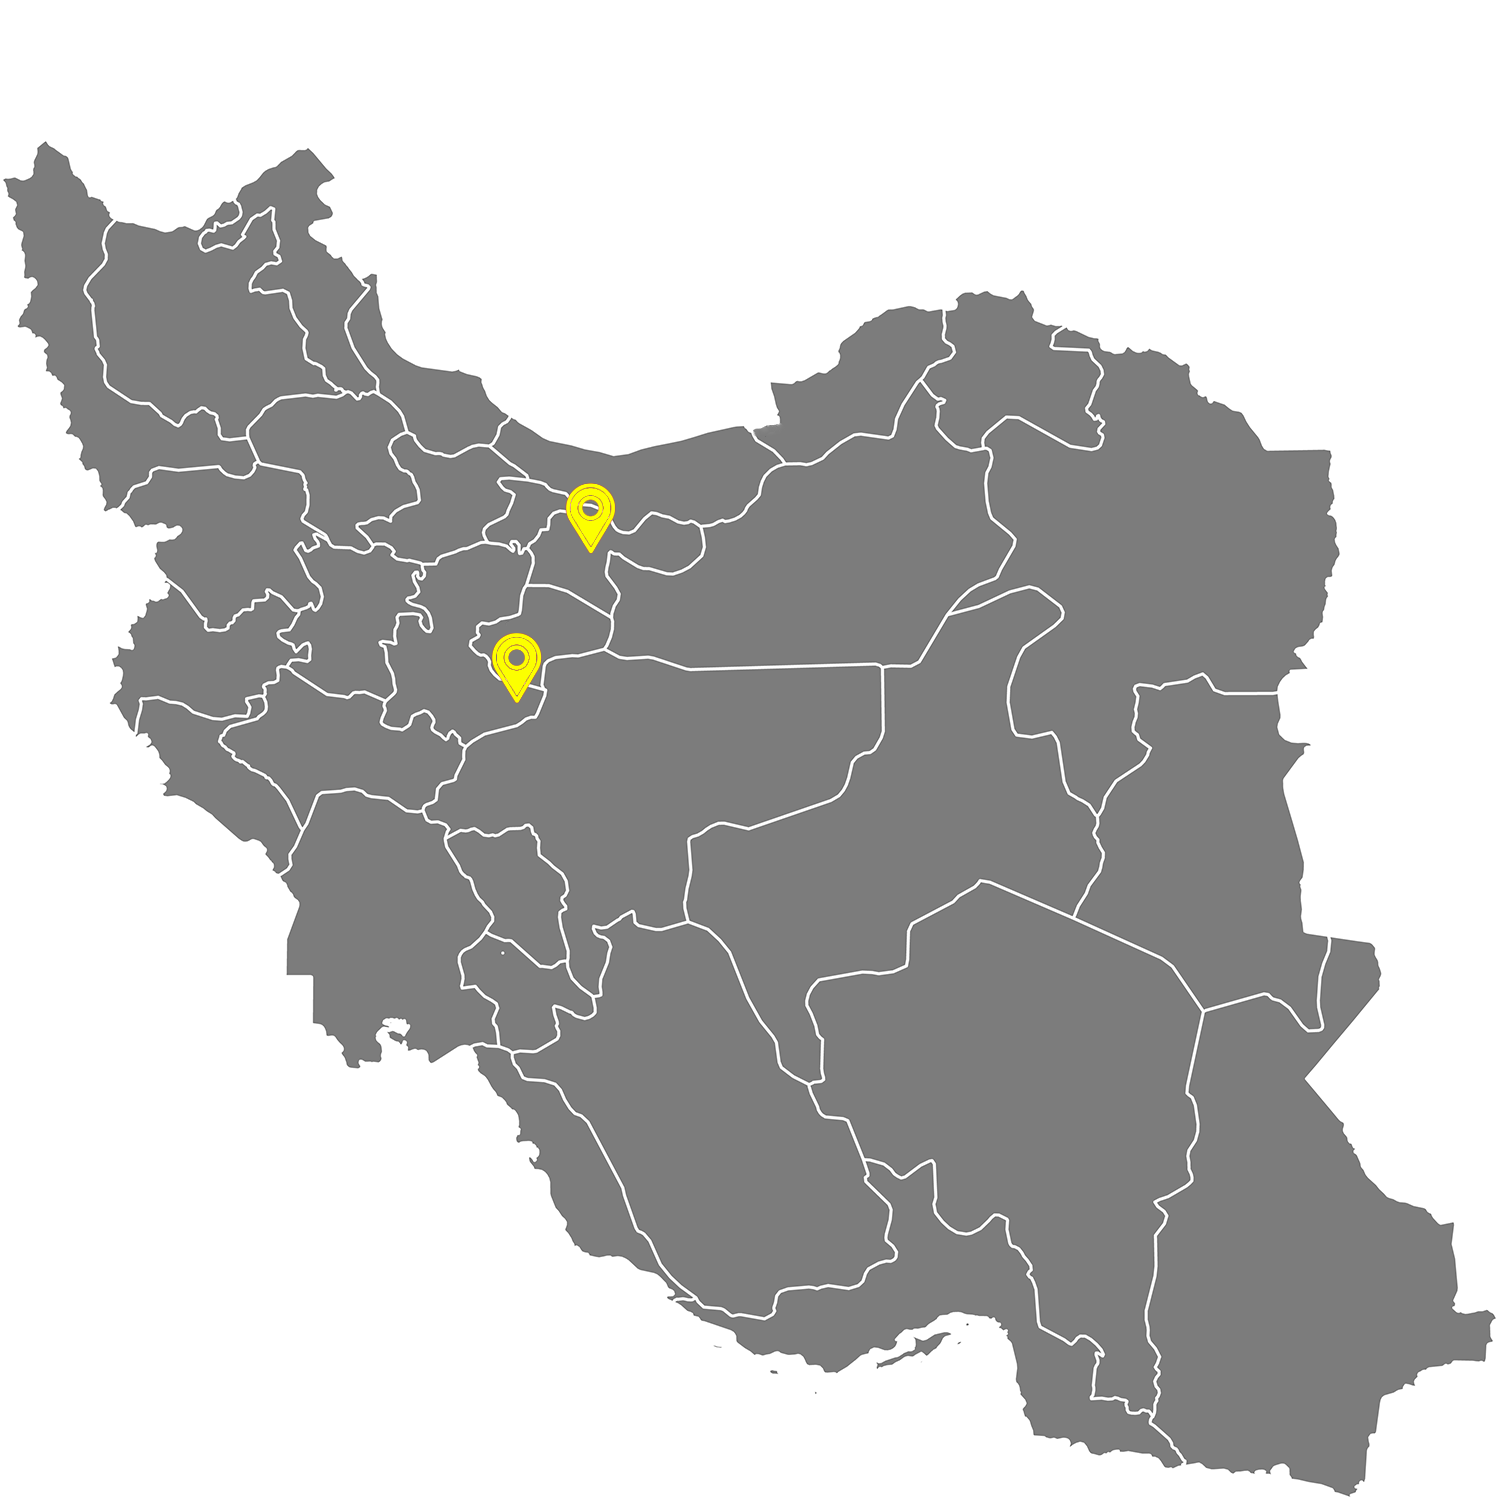
\includegraphics[scale=0.7]{img/iran.png}
    ~
  \section{Languages}
   % \textbf{Italian}
\includegraphics[scale=0.40]{img/5stars.png}
    \textbf{English}
\includegraphics[scale=0.40]{img/2stars.png}
    ~
\end{aside}

\section{Publications}
Author, Author, Author\\
\textbf{Lorem ipsum dolor sit amet, consectetur adipiscing elit, sed do eiusmod tempor incididunt ut labore et dolore magna aliqua}\\
\emph{Lorem ipsum dolor sit amet, consectetur adipiscing elit, sed do eiusmod tempor incididunt ut labore et dolore magna aliqua}
\\
\section{Honors \& Awards}
\begin{entrylist}
  \entry
    {10/2015}
    {''MOMTAZ'' degree in calligraphy}
    {Iran Calligraphers Association}
    {Lorem ipsum.\\
    \emph{Lorem ipsum}}

      \entry
    {10/2015}
    {Holds a patent for invention of ''GHALAMGIR KHOSHNEVISI''}
    {Iranian Patent Office}
    {Lorem ipsum.\\
    \emph{Lorem ipsum}}

          \entry
    {10/2015}
    {Holds a patent for invention of ''DAMABAN SAMA''}
    {Iranian Patent Office}
    {Lorem ipsum.\\
    \emph{Lorem ipsum}}

              \entry
    {10/2015}
    {The first rank in the provincial section and the country's highest rank'}
    {Kharazmi Festival}
    {Lorem ipsum.\\
    \emph{Lorem ipsum}}
\end{entrylist}
\section{Certifications}
\begin{entrylist}
  \entry
    {02/2013}
    {Intro to Computer Science}
    {Udacity. E-learning}
    {\emph{Building a Python Search Engine}}
\end{entrylist}

\section{Other Info}
For the Italian job market:\\
\emph{Si autorizza il trattamento delle informazioni contenute nel curriculum in conformità alle disposizioni previste dal d.lgs. 196/2003. Si dichiara altresì di essere consapevole che, in caso di dichiarazioni non veritiere, si è passibili di sanzioni penali ai sensi del DPR 445/00 oltre alla revoca dei benefici eventualmente percepiti.}
\\
\begin{flushleft}
\emph{May 8th, 2016}
\end{flushleft}
\begin{flushright}
\emph{Ali Heydari}
\end{flushright}

\end{document}
